\noindent
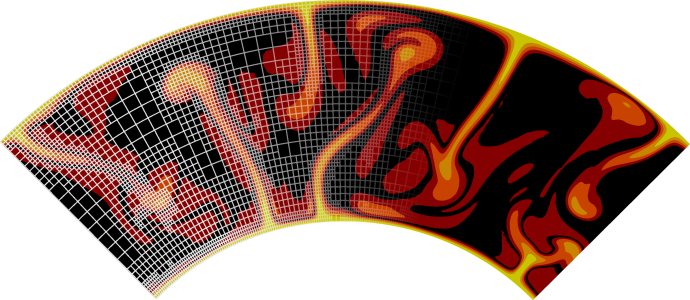
\includegraphics[height=1.25cm]{images/pictograms/aspect_logo}

\includegraphics[height=1.25cm]{images/pictograms/benchmark}

\includegraphics[height=1.25cm]{images/pictograms/under_construction}

\includegraphics[height=1.25cm]{images/pictograms/FEM}

\includegraphics[height=1.25cm]{images/pictograms/paraview}

%%%%%%%%%%%%%%%%%%%%%%%%%%%%%%%%%%%%%%%%%%%%%%%%%%%%%%%%%%%%%%%%%%%%%%%%%%%%%%%%%%%%%%%%%%%%%%%%%%%

\begin{flushright} {\tiny {\color{gray} python\_codes/fieldstone\_175/text.tex}} \end{flushright}

%\lstinputlisting[language=bash,basicstyle=\small]{python_codes/template_keywords.key}

\par\noindent\rule{\textwidth}{0.4pt}

\begin{center}
\inpython
{\small Code: \url{https://github.com/cedrict/fieldstone/tree/master/python_codes/fieldstone_175}}
\end{center}

\par\noindent\rule{\textwidth}{0.4pt}

{\sl This stone was developed with input from Menno Fraters}. \index{contributors}{M. Fraters}

\par\noindent\rule{\textwidth}{0.4pt}

Last revision: June 19th, 2025.

\par\noindent\rule{\textwidth}{0.4pt}

%%%%%%%%%%%%%%%%%%%%%%%%%%%%%%%%%%%%%%%%%%%%%%%%%%%%%%%%%%%%%%%%%%%%%%%%%%%%%%%%%%%%%%%%%%%%%%%%%%%



Our goal here is to introduce dilation in the governing equations.
Dilation implies a change in volume, which conflicts with the assumption of incompressibility. 
Nevertheless we find ourselves wanting to keep using the framework of incompressibility and 
so wish to account for the effects of dilation in the rhs of the mass and momentum conservation
equations. This is very similar to the dilation rate terms of \textcite{chpe15} (2015).

Let us denote by $\vec{\upnu}^0$ and $p$ the solution of the 
incompressible Stokes equations:
\begin{eqnarray}
\vec\nabla \cdot [2  \dot{\bm \varepsilon}^d(\vec\upnu^0)  ]  
-\vec\nabla p + \rho \vec{g} &=& \vec{0} \label{eq:dil1}
\end{eqnarray}
\[
\vec\nabla \cdot \vec\upnu^0 = 0
\]
Let us now consider the velocity field $\vec{\upnu}=\vec{\upnu}^0+\vec{\upnu}_d$
where $\vec{\upnu}_d$ is a user-defined velocity field function that is in $C^2$. 
We assume 2d Cartesian coordinates in $\Omega$, a domain of size $L_x \times L_y$. 

%--------------------------------------
\subsection*{A first simple approach}

For now, let us take $\vec{\upnu}_d=(u_d(x,y) ,0)$.
The strain rate tensor is then given by 
\[
\dot{\bm \varepsilon}(\vec\upnu)= \dot{\bm \varepsilon}(\vec\upnu^0)
+ \dot{\bm \varepsilon}(\vec\upnu_d)= 
\dot{\bm \varepsilon}(\vec\upnu^0) + 
\begin{pmatrix}
\frac{\partial u_d}{\partial x} & \frac12 \frac{\partial u_d}{\partial y}  \\
\frac12 \frac{\partial u_d}{\partial y}  & 0
\end{pmatrix}
\]
Then 
\[
\vec\nabla \cdot \vec\upnu 
= \text{Tr}[\dot{\bm \varepsilon}(\vec\upnu)]
= \underbrace{\text{Tr}[\dot{\bm \varepsilon}(\vec\upnu^0)]}_{=0}
+ \text{Tr}[\dot{\bm \varepsilon}(\vec\upnu_d)]
= \frac{\partial u_d}{\partial x}
\]
This completes the search of the right hand side of the mass conservation equation.

We will also need the corresponding deviatoric strain rate tensor ($D=3$, see discussions in Aspect on the topic
as \url{https://aspect-documentation.readthedocs.io/en/latest/user/methods/basic-equations/2d-models.html}):
\[
\dot{\bm \varepsilon}^d(\vec\upnu_d)
=\dot{\bm \varepsilon}(\vec\upnu_d) - \frac{1}{D} Tr[\dot{\bm \varepsilon}(\vec\upnu_d)] {\bm 1}
=\dot{\bm \varepsilon}(\vec\upnu_d) - \frac{1}{D} \frac{\partial u_d}{\partial x} {\bm 1}
=
\begin{pmatrix}
(1-\frac1D) \frac{\partial u_d}{\partial x} & \frac12 \frac{\partial u_d}{\partial y}  \\
\frac12 \frac{\partial u_d}{\partial y}  & -\frac1D \frac{\partial u_d}{\partial x}
\end{pmatrix}
\]
We now wish to look at the momentum conservation equation with an additional rhs vector term accounting for the dilation:
\[
\vec\nabla \cdot [2 \eta \dot{\bm \varepsilon}^d(\vec\upnu)]  -\vec\nabla p + \rho \vec{g} = \vec{f}_d
\]
First, let us take $\eta=1$ to simplify the equation:
\[
\vec\nabla \cdot [2  \dot{\bm \varepsilon}^d(\vec\upnu)]  -\vec\nabla p + \rho \vec{g} = \vec{f}_d
\]
or,
\[
\vec\nabla \cdot [2  (\dot{\bm \varepsilon}^d(\vec\upnu^0) +\dot{\bm \varepsilon}^d(\vec\upnu_d) ) ]  
-\vec\nabla p + \rho \vec{g} = \vec{f}_d
\]
Using Eq.~\eqref{eq:dil1} the equation above then simply becomes
\[
\vec\nabla \cdot [2  \dot{\bm \varepsilon}^d(\vec\upnu_d)  ]  = \vec{f}_d
\]
or, 
\[
(\partial_x \quad \partial_y) \cdot \begin{pmatrix}
(2-\frac2D) \frac{\partial u_d}{\partial x} &  \frac{\partial u_d}{\partial y}  \\
 \frac{\partial u_d}{\partial y}  & -\frac2D \frac{\partial u_d}{\partial x}
\end{pmatrix}
=(f_x \quad f_y)
\]
i.e., 
\begin{eqnarray}
f_x &=& (2-\frac2D) \frac{\partial^2 u_d}{\partial x^2}  +  \frac{\partial^2 u_d}{\partial y^2} \nn\\
f_y &=& (1-\frac2D) \frac{\partial^2 u_d}{\partial x \partial y}  \label{f175:fxfy}
\end{eqnarray}
We here make the convenient assumption that $u_d$ is only a function of $x$, so that now
\begin{eqnarray}
f_x &=& (2-\frac2D) \frac{\partial^2 u_d}{\partial x^2}   \nn\\
f_y &=& 0
\end{eqnarray}

We have to read this all as follows: There is a dilation term $\frac{\partial u_d}{\partial x}$ 
which is a function of the $x$-coordinate which in turn generates a horizontal flow $(u_d,0)$
atop the Stokes solution $\vec\upnu^0$.

{\color{red} Try later: keep $u_d(x,y)$, also $v_d$ ? }

%-------------------------------------------
\subsection*{A quick remark}

One could think of choosing the dilation rate $du_d/dx$ to be constant in a band and 
zero elsewhere. However, this poses a problem: the rhs of the momentum equation 
contains the term $d^2u_d/dx$, i.e. the gradient of the dilation. That quantity is ill 
defined on the edges of the band. 

One could then prescribe the dilation rate on the nodes and use the basis functions derivatives
to compute (an approximation of) the gradient of the dilation rate. This needs to be tested!

%---------------------------------
\subsection*{weak form}

There is no real difficulty in establishing the weak form 
of the mass and momentum conservation equations with the additional rhs terms. 

By considering $\rho\vec{g}-\vec{f}_d$ as a single vector we have virtually nothing to do 
in the momentum equation. 
In the case of the mass equation, we have a rhs that poses no difficulty 
\[
\int_\Omega \vec{\bN}^p \frac{\partial u_d}{\partial x}  dV
\]
Both terms are already present in Aspect (plastic dilation term implemented by Timo, John and me).

In terms of implementation, we need to make sure that the matrix entering the $\K$ block is defined as 
follows:
\begin{lstlisting}
c_mat = np.array([[4/3,-2/3,0],[-2/3,4/3,0],[0,0,1]],dtype=np.float64) 
...
K_el+=b_mat.T.dot(c_mat.dot(b_mat))*eta*weightq*jcob
\end{lstlisting}
The rhs terms are simply:
\begin{lstlisting}
for i in range(0,mV):
    f_el[ndofV*i+0]+=NNNV[i]*jcob*weightq*(rho*gx(xq,yq)-d2uddx2(xq,yq,Lx,Ly)*(2-2./3))
    f_el[ndofV*i+1]+=NNNV[i]*jcob*weightq*(rho*gy(xq,yq)-0)

h_el[:]-=NNNP[:]*duddx(xq,yq,Lx,Ly)*weightq*jcob
\end{lstlisting}

The required functions for the 2 following experiments are defined as follows:
\begin{lstlisting}
def ud(x,y,Lx,Ly):
    if experiment==1:
       return 0.5*(x-Lx/2 -Lx/2/np.pi*np.sin(2*np.pi*x/Lx) )
    if experiment==2:
       delta=Lx/8
       if x<=Lx/2-delta: 
          return -delta/2
       elif x<=Lx/2+delta:
          return 0.5*(x-Lx/2+delta/np.pi*np.sin(np.pi*(x-Lx/2)/delta))
       else: 
          return delta/2

def duddx(x,y,Lx,Ly):
    if experiment==1:
       return (1-np.cos(2*np.pi*x/Lx))/2
    if experiment==2:
       delta=Lx/8
       if abs(x-Lx/2)<=delta: 
          return 0.5*(1+np.cos(np.pi*(x-Lx/2)/delta))
       else:
          return 0

def d2uddx2(x,y,Lx,Ly):
    if experiment==1:
       return np.pi/Lx*np.sin(2*np.pi*x/Lx)
    if experiment==2:
       delta=Lx/8
       if abs(x-Lx/2)<=delta: 
          return -0.5*np.pi/delta*np.sin(np.pi*(x-Lx/2)/delta)
       else:
          return 0
\end{lstlisting}


%--------------------------------------------------------------
\subsection*{Simple case of a vertical cosine hill dilation zone (experiment \#1)}

It feels more natural to postulate a dilation zone and then compute the corresponding velocity
than the other way around, so we set
\[
\frac{d u_d}{d x} = \frac12 (1-\cos(\frac{2 \pi x}{L}))
\]
i.e., the dilation zone is strong in the middle of the domain and zero on the sides. 
The dilation velocity $u_d(x)$ is then given by integration of the equation above
\[
u_d(x) = \frac12x - \frac{L}{4\pi  }\sin (\frac{2 \pi x}{L}) +C
\]
where $C$ is the integration constant.
Given the planar symmetry $u_d$ should be zero along the line $x=L_x/2$, so 
\[
0 = \frac{L}{4}  + C \qquad \Rightarrow \qquad C = -L/4
\]
Then in the end:
\[
u_d(x) = \frac12 \left( x- \frac{L}{2} - \frac{L}{2\pi }\sin (\frac{2 \pi x}{L}) \right)
\]
Finally we will also need
\[
\frac{d^2 u_d}{d x^2} = \frac{\pi}{L}  \sin(\frac{2 \pi x}{L})
\]
The analytical expressions for $u_d$ and $du_d/dx$ are shown here:
\begin{center}
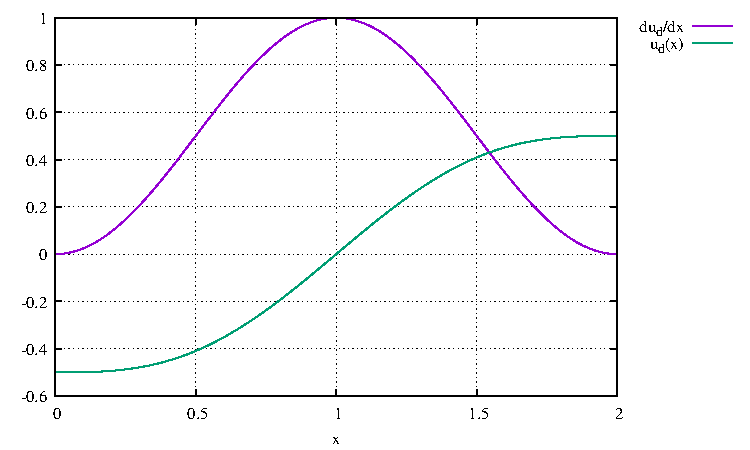
\includegraphics[width=8cm]{python_codes/fieldstone_175/results/exp1/analytical.pdf}\\
{\captionfont dilation term and resulting velocity fields.}
\end{center}



\begin{center}
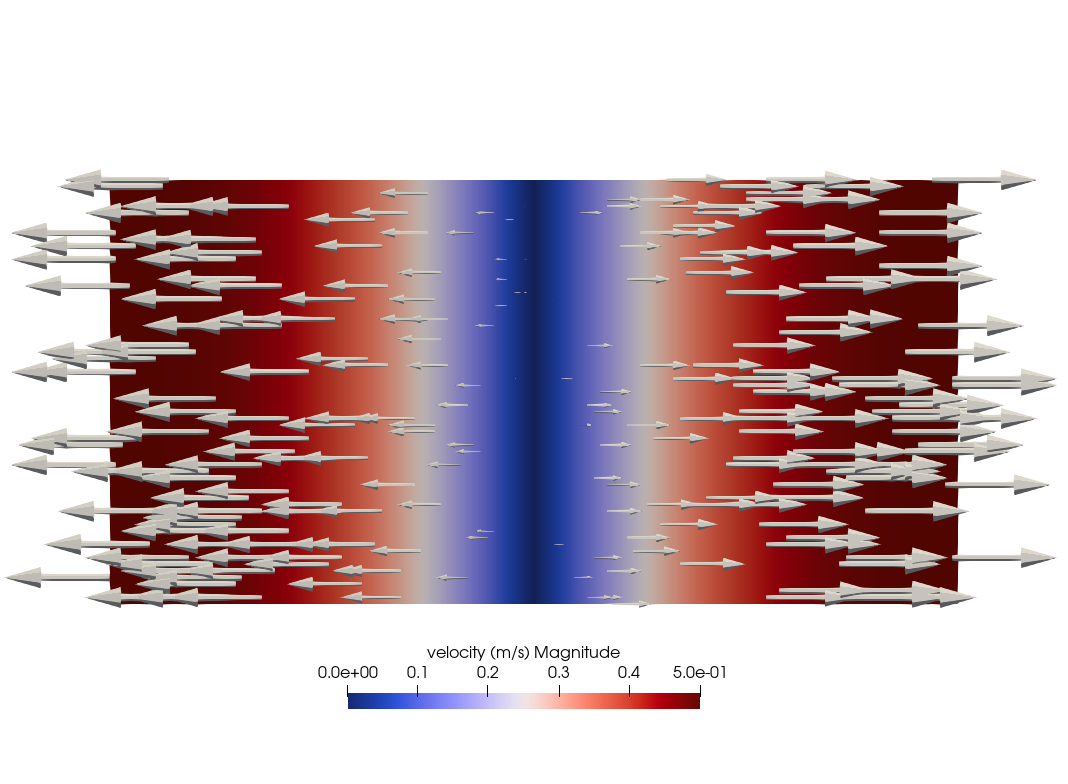
\includegraphics[width=8cm]{python_codes/fieldstone_175/results/exp1/ud.png}
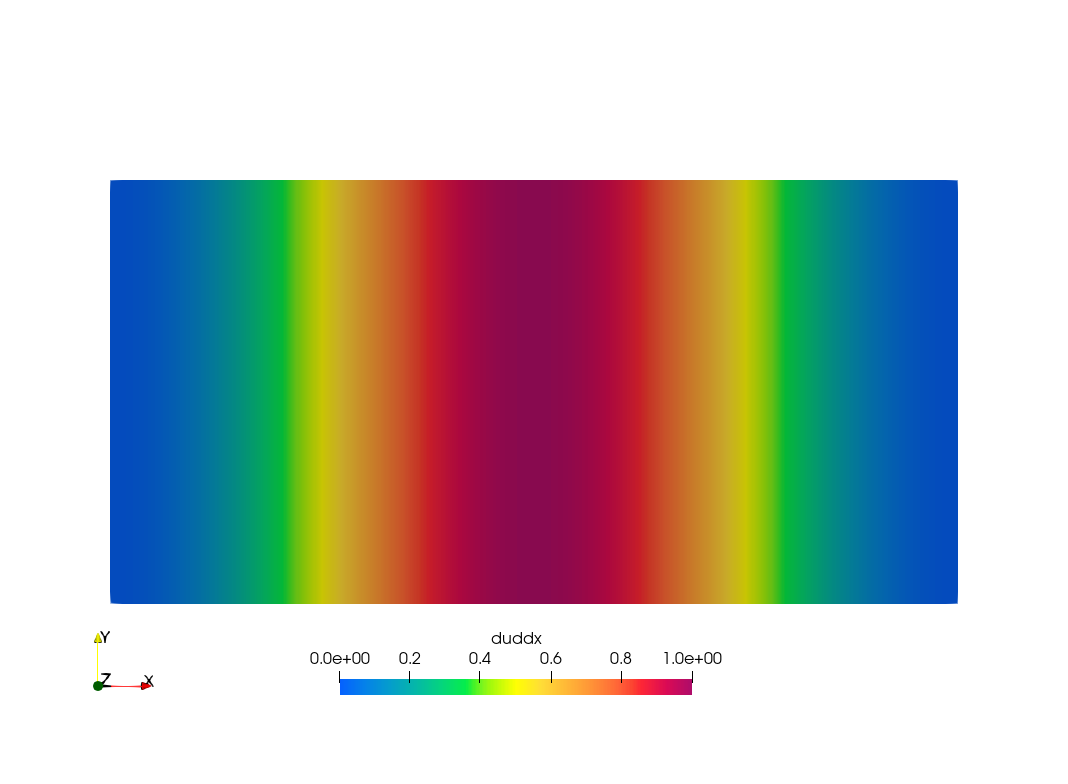
\includegraphics[width=8cm]{python_codes/fieldstone_175/results/exp1/duddx.png}\\
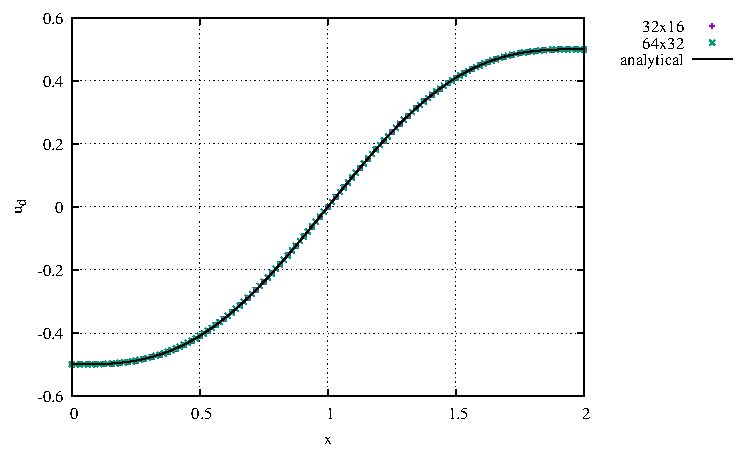
\includegraphics[width=8cm]{python_codes/fieldstone_175/results/exp1/ud.pdf}\\
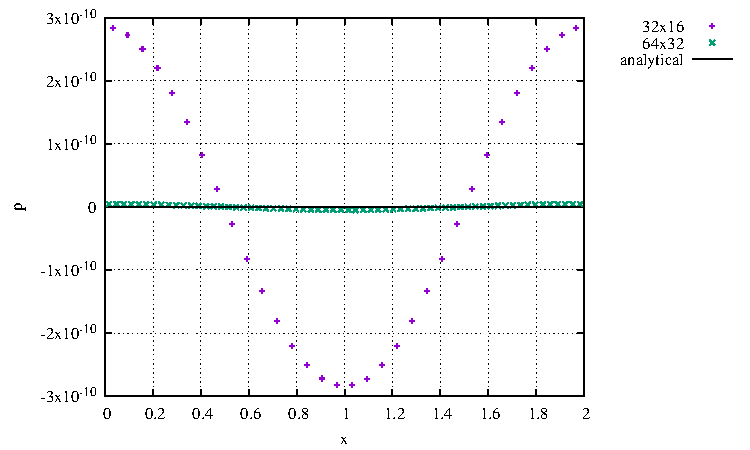
\includegraphics[width=8cm]{python_codes/fieldstone_175/results/exp1/p.pdf}
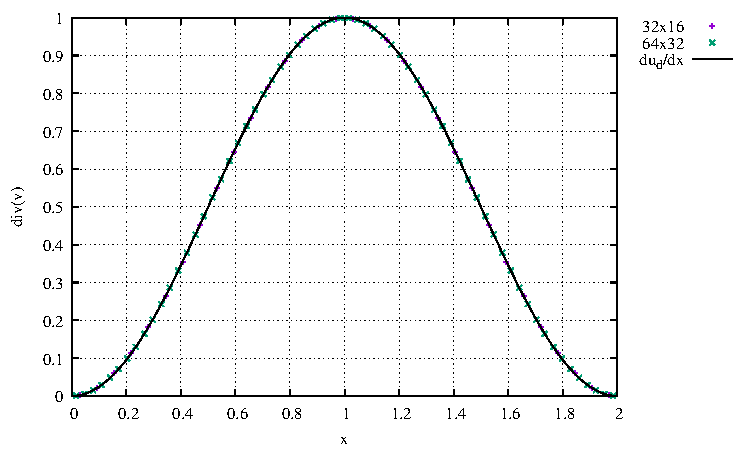
\includegraphics[width=8cm]{python_codes/fieldstone_175/results/exp1/divv.pdf}\\
{\captionfont Results obtained with the code for 2 different resolutions.}
\end{center}

%-----------------------------------------------------------------------------------
\subsection*{Simple case of a vertical cosine hill dilation zone (experiment \#2)}

We now start from a different dilation zone:
\[
\frac{d u_d}{d x} = \frac12 (1+\cos\frac{ \pi (x-L/2)}{\delta})
\]
for $|x-Lx/2|<\delta$, zero otherwise.
We then integrate to find
\[
u_d(x) = \frac12x + \frac12\frac{\delta }{\pi  }\sin  \frac{ \pi (x-L/2)}{\delta} +C
\]
we find again $C=-L/4$
so that 
\[
u_d(x) = \frac12 \left[ x-L/2 + \frac{\delta }{\pi  }\sin  \frac{ \pi (x-L/2)}{\delta} \right]
\]
for $|x-Lx/2|<\delta$. Outside, we have
$u_d=constant$. We of course require the velocity to be continuous at 
$x=L/2\pm \delta$ with:
\[
u_d(x=L/2+\delta) = \frac{\delta }{2} 
\qquad
u_d(x=L/2-\delta) = -\frac{\delta }{2} 
\]
Finally we will need
\[
\frac{d^2 u_d}{d x^2} = -\frac{\pi}{2\delta}  \sin \frac{ \pi (x-L/2)}{\delta}
\]
The analytical expressions for $u_d$ and $du_d/dx$ are shown here:
\begin{center}
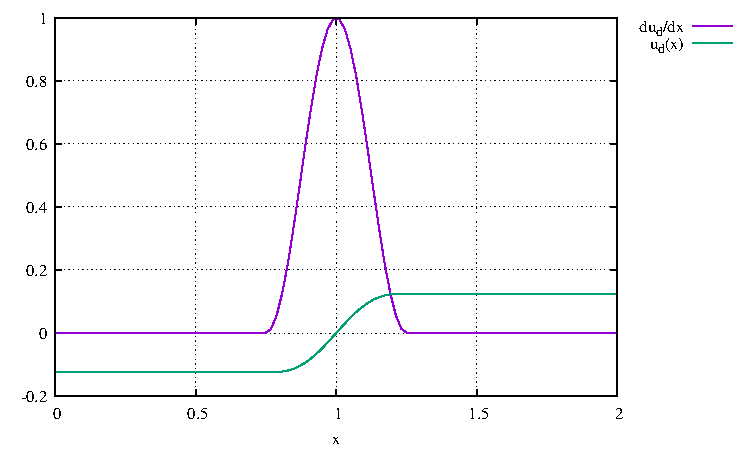
\includegraphics[width=8cm]{python_codes/fieldstone_175/results/exp2/analytical.pdf}\\
{\captionfont dilation term and resulting velocity fields.}
\end{center}

As above we set $L_x=2$, $L_y=1$. Free slip boundary conditions are imposed on the 
top and bottom boundaries. $u=0$ is also presribed at location $(x=L_x/2,y=L_y)$
so as to remove the translational nullspace. $\rho$ is set to zero and $\eta=1$. 
In the absence of dilation rate, the Stokes solution is then a zero velocity field and pressure field.

\begin{center}
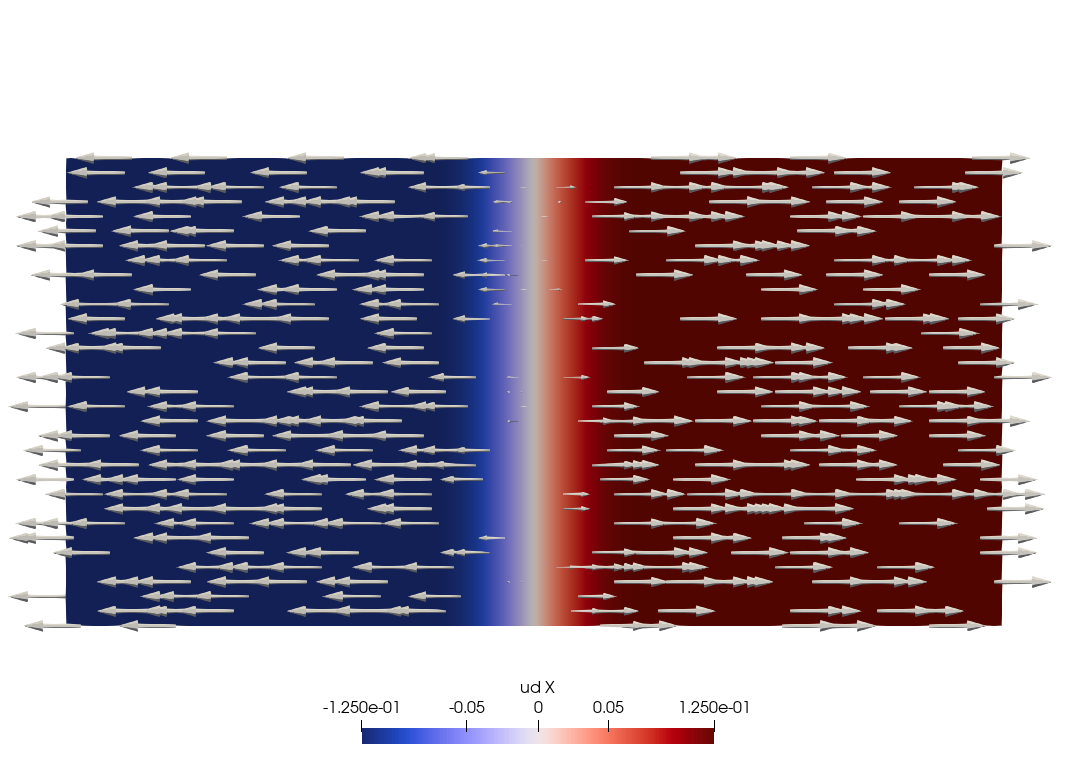
\includegraphics[width=8cm]{python_codes/fieldstone_175/results/exp2/ud.png}
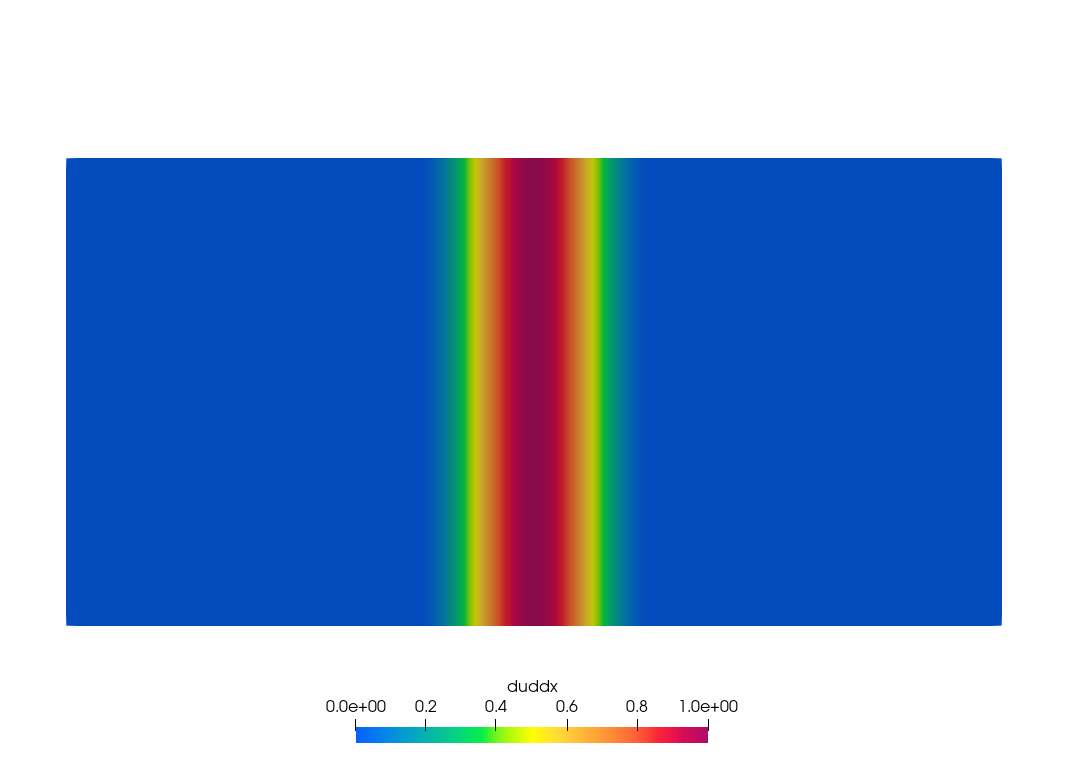
\includegraphics[width=8cm]{python_codes/fieldstone_175/results/exp2/duddx.png}\\
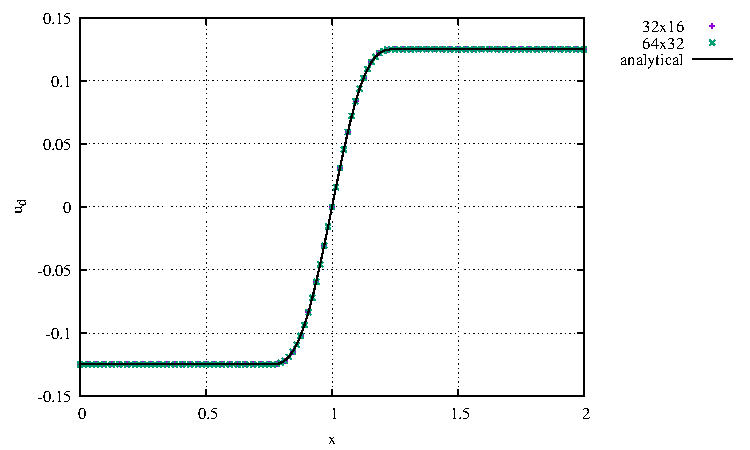
\includegraphics[width=8cm]{python_codes/fieldstone_175/results/exp2/ud.pdf}\\
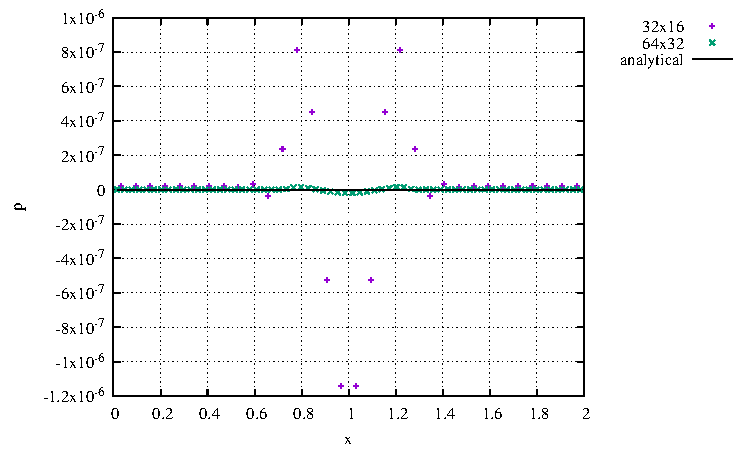
\includegraphics[width=8cm]{python_codes/fieldstone_175/results/exp2/p.pdf}
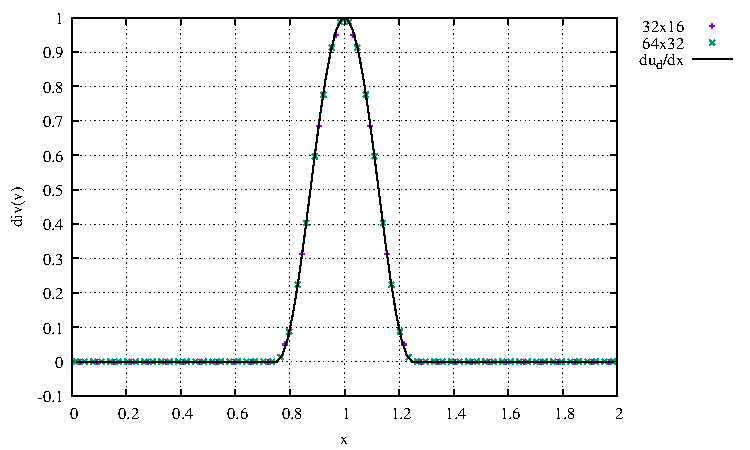
\includegraphics[width=8cm]{python_codes/fieldstone_175/results/exp2/divv.pdf}\\
{\captionfont Results obtained with the code for 2 different resolutions.}
\end{center}


\newpage
%--------------------------------------
\subsection*{A not so simple approach}

Let us now take $\vec{\upnu}_d=(u_d(x,y) , v_d(x,y))$.
The strain rate tensor is then given by 
\[
\dot{\bm \varepsilon}(\vec\upnu)
= \dot{\bm \varepsilon}(\vec\upnu^0) + \dot{\bm \varepsilon}(\vec\upnu_d)
= \dot{\bm \varepsilon}(\vec\upnu^0) 
+ 
\begin{pmatrix}
\frac{\partial u_d}{\partial x} & \frac12 (\frac{\partial u_d}{\partial y}+ \frac{\partial v_d}{\partial x})  \\
\frac12 (\frac{\partial u_d}{\partial y}+ \frac{\partial v_d}{\partial x})  & \frac{\partial v_d}{\partial y}
\end{pmatrix}
\]
Then 
\[
\vec\nabla \cdot \vec\upnu 
= \text{Tr}[\dot{\bm \varepsilon}(\vec\upnu)]
= \underbrace{\text{Tr}[\dot{\bm \varepsilon}(\vec\upnu^0)]}_{=0}
+ \text{Tr}[\dot{\bm \varepsilon}(\vec\upnu_d)]
= \frac{\partial u_d}{\partial x} + \frac{\partial v_d}{\partial y}
\]
This completes the search of the right hand side of the mass conservation equation.

We continue with the corresponding deviatoric strain rate tensor 
\begin{eqnarray}
\dot{\bm \varepsilon}^d(\vec\upnu_d)
&=&\dot{\bm \varepsilon}(\vec\upnu_d) - \frac{1}{D} Tr[\dot{\bm \varepsilon}(\vec\upnu_d)] {\bm 1} \nn\\
&=&\dot{\bm \varepsilon}(\vec\upnu_d) - \frac{1}{D} (\frac{\partial u_d}{\partial x} + \frac{\partial v_d}{\partial y}) {\bm 1} \nn\\
&=&
\begin{pmatrix}
\frac{\partial u_d}{\partial x}- \frac{1}{D} (\frac{\partial u_d}{\partial x} + \frac{\partial v_d}{\partial y})
& \frac12 (\frac{\partial u_d}{\partial y}+ \frac{\partial v_d}{\partial x})  \\
\frac12 (\frac{\partial u_d}{\partial y}+ \frac{\partial v_d}{\partial x})  
& \frac{\partial v_d}{\partial y} - \frac{1}{D} (\frac{\partial u_d}{\partial x} + \frac{\partial v_d}{\partial y})
\end{pmatrix} \nn\\
&=& 
\begin{pmatrix}
(1-\frac{1}{D}) \frac{\partial u_d}{\partial x}- \frac{1}{D} \frac{\partial v_d}{\partial y}
& \frac12 (\frac{\partial u_d}{\partial y}+ \frac{\partial v_d}{\partial x})  \\
\frac12 (\frac{\partial u_d}{\partial y}+ \frac{\partial v_d}{\partial x})  
& -\frac{1}{D} \frac{\partial u_d}{\partial x} + (1- \frac{1}{D})  \frac{\partial v_d}{\partial y} 
\end{pmatrix} \nn
\end{eqnarray}

We set again $\eta=1$ to simplify the equations. We then have 

\[
\vec{f}_d = \vec\nabla \cdot [2  \dot{\bm \varepsilon}^d(\vec\upnu_d)  ]  
\]

\[
(\partial_x \quad \partial_y) \cdot 2  
\begin{pmatrix}
(1-\frac{1}{D}) \frac{\partial u_d}{\partial x}- \frac{1}{D} \frac{\partial v_d}{\partial y}
& \frac12 (\frac{\partial u_d}{\partial y}+ \frac{\partial v_d}{\partial x})  \\
\frac12 (\frac{\partial u_d}{\partial y}+ \frac{\partial v_d}{\partial x})  
& -\frac{1}{D} \frac{\partial u_d}{\partial x} + (1- \frac{1}{D})  \frac{\partial v_d}{\partial y} 
\end{pmatrix} 
=(f_x \quad f_y)
\]
or, 
\begin{eqnarray}
\frac12 f_x(x,y) &=&  (1-\frac{1}{D}) \frac{\partial^2 u_d}{\partial x^2}- \frac{1}{D} \frac{\partial^2 v_d}{\partial x\partial y} 
+ \frac12 (\frac{\partial^2 u_d}{\partial y^2}+ \frac{\partial^2 v_d}{\partial x \partial y}) \nn\\
\frac12 f_y(x,y) &=& \frac12 (\frac{\partial^2 u_d}{\partial x \partial y}+ \frac{\partial^2 v_d}{\partial x^2})
 -\frac{1}{D} \frac{\partial^2 u_d}{\partial x \partial y} + (1- \frac{1}{D})  \frac{\partial^2 v_d}{\partial y^2} 
\end{eqnarray}
and finally

\begin{eqnarray}
f_x(x,y) &=&  (2-\frac{2}{D}) \frac{\partial^2 u_d}{\partial x^2}
+  \frac{\partial^2 u_d}{\partial y^2}
+ (1 - \frac{2}{D}) \frac{\partial^2 v_d}{\partial x\partial y}  \nn\\
f_y(x,y) &=& (1 - \frac{2}{D}) \frac{\partial^2 u_d}{\partial x\partial y} 
+ \frac{\partial^2 v_d}{\partial x^2} + (2-\frac{2}{D}) \frac{\partial^2 v_d}{\partial y^2}
\end{eqnarray}

We can verify that these expressions are identical to Eq.~\eqref{f175:fxfy} when $v_d=0$.

In order to build a concrete case the difficulty lies in the fact that we must now 
choose $u_d(x,y)$ and $v_d(x,y)$.
Let us now postulate 

\[
u_d(x,y) = \frac12 \left[ x-L/2 + \frac{\delta }{\pi  }\sin  \frac{ \pi (x-L/2)}{\delta} \right]
\sin \frac{\pi y}{L_y}
\]
\[
v_d(x,y)
\]







